
\documentclass[tikz,border=5pt]{standalone}

% Core packages
\usepackage{amsmath,amssymb}
\usepackage{tikz}
\usepackage{tikz-cd}
\usepackage{pgfplots}
\usepackage{multicol}
\usepackage{xcolor}
\usepackage{caption}
\usepackage{float}
\usepackage{kotex}

% TikZ / PGF configuration
\usetikzlibrary{
  arrows.meta,
  calc,
  positioning,
  shapes.geometric,
  shapes.symbols,
  fit,
  backgrounds,
  patterns,
  matrix,
  intersections,
  decorations.pathmorphing,
  decorations.markings,
  angles,
  quotes
}
\pgfplotsset{compat=1.18}

% Reusable TikZ styles
\tikzset{
  >=stealth,
  line cap=round,
  line join=round,
  every picture/.style={line width=0.9pt},
  box/.style={draw, rounded corners, minimum width=2.8cm, minimum height=1.2cm, align=center},
  circlebox/.style={draw, circle, minimum size=1cm, align=center},
  arrow/.style={->, thick},
  dashedarrow/.style={->, thick, dashed},
  point/.style={circle, fill, inner sep=1.2pt},
  gridhelp/.style={help lines, gray!35},
  highlight/.style={fill=blue!10, draw=blue!60!black},
  3D/.style={
    x={(-0.60cm,-0.42cm)},
    y={(0.78cm,0cm)},
    z={(0cm,0.78cm)}
  }
}


\begin{document}

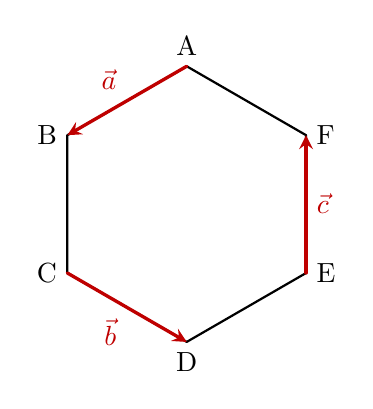
\begin{tikzpicture}[scale=1.75, line cap=round, line join=round]
  \pgfmathsetmacro{\rt}{sqrt(3)/2}

  \coordinate (A) at (0,1);
  \coordinate (B) at (-\rt,0.5);
  \coordinate (C) at (-\rt,-0.5);
  \coordinate (D) at (0,-1);
  \coordinate (E) at (\rt,-0.5);
  \coordinate (F) at (\rt,0.5);

  \draw[thick] (A)--(B)--(C)--(D)--(E)--(F)--cycle;

  \draw[-stealth, very thick, red!75!black] (A)--(B)
    node[midway, above left] {$\vec a$};
  \draw[-stealth, very thick, red!75!black] (C)--(D)
    node[midway, below left] {$\vec b$};
  \draw[-stealth, very thick, red!75!black] (E)--(F)
    node[midway, right] {$\vec c$};


  \node[above] at (A) {$\mathrm{A}$};
  \node[left] at (B) {$\mathrm{B}$};
  \node[left] at (C) {$\mathrm{C}$};
  \node[below] at (D) {$\mathrm{D}$};
  \node[right] at (E) {$\mathrm{E}$};
  \node[right] at (F) {$\mathrm{F}$};
\end{tikzpicture}

\end{document}

